\documentclass[PhD]{dukethesis2006}

%preamble here for options

%-----------------------------------------------------------------------------%
% DEFINITIONS:
%
% include \usepackage here
%-----------------------------------------------------------------------------%
\usepackage{amsmath}
\usepackage{amssymb}
\usepackage{amsthm}
\usepackage{array}
\usepackage{epsfig}
\usepackage{graphicx}
\usepackage{xy}

%----  macros to save typing; added by hartley, 2002 ----
\newcommand{\fig}{\begin{figure}[htbp]\centering}
\newcommand{\pic}[1]{\includegraphics[width=#1]}
\newcommand{\efig}{\end{figure}} 
%\newcommand{\efig}{\end{figure} \clearpage}
% Use \clearpage to cure ``too many floats'' problem (1 fig. per page).
\newcommand{\fr}[1]{Figure \ref{fig:#1}}
\newcommand{\FR}[1]{Figure \ref{fig:#1}}
\newcommand{\er}[1]{equation \ref{eq:#1}}
\newcommand{\ER}[1]{Equation \ref{eq:#1}}
\newcommand{\eq}{\begin{equation}}
\newcommand{\eeq}{\end{equation}}
\newcommand{\eqa}{\begin{eqnarray}}
\newcommand{\eeqa}{\end{eqnarray}}
\newcommand{\etal}{\nobreak\mbox{\it et al.}}



% \newcommand{\singlespacing}{%
%   \let\CS=\small\renewcommand{\baselinestretch}{1.0}\CS}
% \newcommand{\doublespacing}{%
%   \let\CS=\small\renewcommand{\baselinestretch}{1.6}\CS}
% \newcommand{\normalspacing}{\doublespacing}

%\newcommand{\singlespacingplus}{%
%  \let\CS=\@currsize\renewcommand{\baselinestretch}{1.25}\tiny\CS}
%\newcommand{\realdoublespacing}{%
%  \let\CS=\@currsize\renewcommand{\baselinestretch}{2}\tiny\CS}
%\newcommand{\footnotespacing}{\singlespacing}
%\newcommand{\changespacing}[2]{%
%  \renewcommand{#1}{%
%    \let\CS=\@currsize\renewcommand{\baselinestretch}{#2}\tiny\CS}%
%}
%\newcommand{\changenormalspacing}[1]{\renewcommand{\normalspacing}{#1}}




%---- units ----
\newcommand{\days}{\nobreak\mbox{$\;$days}}
\newcommand{\hrs}{\nobreak\mbox{$\;$hrs}}
\newcommand{\mins}{\nobreak\mbox{$\;$min}}
\newcommand{\s}{\nobreak\mbox{$\;$s}}
\newcommand{\ms}{\nobreak\mbox{$\;$ms}}
\newcommand{\us}{\nobreak\mbox{$\;\mu$s}}
\newcommand{\inch}{\nobreak\mbox{$\;$in}}
\newcommand{\meter}{\nobreak\mbox{$\;$m}}
\newcommand{\cm}{\nobreak\mbox{$\;$cm}}
\newcommand{\mm}{\nobreak\mbox{$\;$mm}}
\newcommand{\um}{\nobreak\mbox{$\;\mu$m}}
\newcommand{\nm}{\nobreak\mbox{$\;$nm}}
\newcommand{\cmpers}{\nobreak\mbox{$\;$cm\,s$^{-1}$}}
\newcommand{\mmpers}{\nobreak\mbox{$\;$mm\,s$^{-1}$}}
\newcommand{\umpers}{\nobreak\mbox{$\;\mu$m\,s$^{-1}$}}
\newcommand{\g}{\nobreak\mbox{$\;$g}}
\newcommand{\kg}{\nobreak\mbox{$\;$kg}}
\newcommand{\hz}{\nobreak\mbox{$\;$Hz}}
\newcommand{\mhz}{\nobreak\mbox{$\;$mHz}}
\newcommand{\uhz}{\nobreak\mbox{$\;\mu$Hz}}


%---- oft-used complicated symbols ----
\newcommand{\rms}{\nobreak\mbox{$\sigma_{rms}$}}
\newcommand{\sat}{\nobreak\mbox{$\sigma_{\textrm{sat}}$}}
\newcommand{\DG}{\nobreak\mbox{$\Delta G^2$}}
\newcommand{\DS}{\nobreak\mbox{$\Delta\sigma$}}
\newcommand{\DQ}{\nobreak\mbox{$\Delta\theta$}}
\newcommand{\DSDQ}{\nobreak\mbox{$\Delta\sigma/\Delta\theta$}}
\newcommand{\dq}{\nobreak\mbox{$d\theta$}}
\newcommand{\ds}{\nobreak\mbox{$d\sigma$}}
\newcommand{\dsdq}{\nobreak\mbox{$d\sigma/d\theta$}}
\newcommand{\YY}{$\curlyvee\curlywedge$}
\newcommand{\GG}{\nobreak\mbox{$G^2$}}

 
% This is where the shortened versions of Latex environments like figure, equation, etc 
% are defined. See the file for the shortcuts.

\author{[Author Name]}
\advisor{[Advisor Name]}
\member{[Committee Member Name]}
\member{[Committee Member Name]}
\member{[Committee Member Name]}
\member{[Committee Member Name]}

\department{[Department Name]}
%\subject{xxx} If this is used, "subject" has to be un-commented in the cls file in several places
\title{[Dissertation Title]}

%end of preamble, beginning of printable document

\begin{document}


\Copyright

\maketitle

\makeabstract

\abstract
This is a template for theses and dissertations at Duke University. It is not intended to demonstrate all the features of \LaTeX, only to provide help with the format of your work. There are numerous very good online references for detailed help with \LaTeX, including a downloadable, fairly exhaustive guide at\\
ftp://ftp.giss.nasa.gov/pub/sgreen/latex/latex.tar.gz.

An abstract is only required in doctoral dissertations. Your complete abstract should be no more than 350 words. In the abstract, you must (1) present the problem of the dissertation, (2) discuss the materials and methods used, and (3) state the conclusions reached. Individual chapters should not have abstracts. The Abstract will be published in Dissertation Abstracts International. Note that this should be the first numbered page: it is page iv; pages i, ii and iii  (copyright, dissertation signature page and abstract signature page) were counted but not numbered. If you look ahead, you will see that numbering up to the first page of text is in roman numerals. On the first page of text in chapter one, numbering restarts at 1. This numbering (1,2,3,4�) is consecutive through the rest of the document. 

\acknowledgements
Hosana pronomeca nelimigita ido ko, us negi lanta leterskribi mal. Re nia panjo alikvante nombrovorto, via tc bisi hekto koruso. Cii go unun oble drumo. Ke ties okej laringalo mia, anti duona alial ing fi. Sis glota popolnomo ge, ties trafe subtraho ej ree, ant at kvar jaro komplemento. It sor tempa oktiliono antaupriskribo.

Modo tiela us cii, ne ehe intere rilativo. Ferio multiplikite id ajn. Tiele nenio akuzativa co ian. Unu ilia longa leteri op, vola hola ge cit, altmontaro kromakcento mi des. Ont lo grupo sezononomo, um kaj elparolo sanskrito.


%A table of contents file is automatically generated in the same folder as the .tex file when
%the \tableofcontents is used
\tableofcontents

\listoffigures

\listoftables

%-----------------------------------------------------------------------------%
% replace FILE in \input{FILE} with name of tex file
% containing the given chapter, eg. for the introduction one could
% have FILE = intro if stored in intro.tex (.tex extension is assumed!).
%-----------------------------------------------------------------------------%

\chapter{Introduction}
\pagenumbering{arabic}

%A large document requires a lot of input. Rather than putting the whole input in a single large file, it's more efficient to split it into several smaller ones. Regardless of how many separate files you use, there is one that is the root file; it is the one whose name you type when you run LaTeX. In this template, the introduction chapter is an external file (intro.tex) and the second chapter is contained internally in the root file (in this file you are reading)
% The \vspace{} command in this chapter is just for aesthetic reasons - I don't like something new to start at the last line 
%of the page

% ONE OF THE BEST ONLINE LATEX REFERENCES IS AT :
% http://www.eng.cam.ac.uk/help/tpl/textprocessing/latex_advanced/latex_advanced.html

%% ALL figures are in EPS format: It is the best possible format 


% The \vspace{} command in this chapter is just for aesthetic reasons - I don't like something new to start at the last line 
%of the page

% ONE OF THE BEST ONLINE LATEX REFERENCES IS AT :
% http://www.eng.cam.ac.uk/help/tpl/textprocessing/latex_advanced/latex_advanced.html

%% ALL figures are in EPS format: It is the best possible format 

\section{Tuberculosis}

Of all the infectious agents to have ever afflicted humankind, \textit{Mycobacterium tuberculosis} is perhaps the most imminently successful. The primary cause of potentially greater than one billion human deaths since 1800 alone (approximately 9\% of all deaths in that time period) (citation), this disease has had profound impact on the cultural and political development of the modern world and continues to impact the lives of most people around the world today\footnote{For additional reading on this subject of how tuberculosis has impacted the development of human society, see (citation).}. Fallaciously considered a disease of antiquity, this disease manifests in active disease in greater than 10 million people each year and has killed greater than one million people per year each year since records or estimates have been available with the case and death burden rising due to health system neglect exposed by the COVID-19 pandemic ongoing at the time of this writing (citation). 

\textit{Mycobacterium tuberculosis} has long been of basic scientific interest on account of the myriad ways in which it undermines host immune responses to establish a replicative niche within the human lung. \textit{M. tuberculosis} infection results in the formation of caseating granulomas encased in a complex network of immune cells within which the bacteria replicate. Over evolutionary time, these bacteria have innovated novel ways of subverting host-protective immune responses while exacerbating maladaptive ones. This makes the study of tuberculosis not only the study of microbiology and immunology, but a fascinating study in the basic principles of cell biology. 

\subsection{History of Tuberculosis}

The overwhelming prevalence of tuberculosis in the 18th and 19th centuries led to an extreme degree of cultural salience for this disease in the daily lives of the people of those times. Responsible for the deaths of many preeminent public figures of these eras\footnote{The number of such public figures is far too great to list. From the 1840s and 1850s alone, tuberculosis was responsible for the deaths of Andrew Jackson (seventh president of the United States), Henry Clay (Secretary of State, Speaker of the House, three-time presidential candidate for the Whig Party), John C. Calhoun (Vice President, Secretary of State), Alexis de Tocqueville (famed French observer of American culture and author of the classic of political theory, Democracy in America), Henry David Thoreau (naturalist author of Walden), and Emily Bront\"{e} (author of Wuthering Heights).}, it is also a ubiquitous feature of the literature of those times as well. Perhaps most famously, tuberculosis is depicted as the disease that afflicts the Lowood School in Charlotte Bront��\"{e}'s Jane Eyre, among other novels depicting the disease then known as \textit{��consumption��} for the way in which it leads to cachexia, increasing pallor, hemoptysis, and ultimately death (citation).

This cachexia is a defining feature of tuberculosis across phylogenies; such progressive wasting unable to be ameliorated by improved nutrition is an unusual presentation strongly reminiscent of many cancers and rather dissimilar from most infectious diseases (citation). Indeed, as medical understanding of diseases progressed beyond concepts of humoral imbalance, a prevailing theory was that tuberculosis was a hereditary form of cancer due to the way it spread within families (citation). The functional and consequential similarities between tuberculosis and cancer are replete and will be a subject returned to throughout this document.

First documented in 1888 by Robert Koch, the tubercle bacillus, Mycobacterium tuberculosis, was a foundational instrument in the broader development of the field of microbiology and remains a major area of research today\footnote{For more on this, see (citation).} (citation). Once thought to have been banished to the annals of history, tuberculosis, after a steady decline in cases throughout the middle of the 20th century\footnote{This was coincident with, but likely unrelated to, the development of effective antibiotic therapies. Indeed, the modern disparity between tuberculosis rates between the United States and Western Europe and much of the rest of the world is thought to have more to do with improved living conditions, growing herd immunity, and improved nutrition rather than the use of antibiotics as downward trends actually began 100 years prior to the discovery of streptomycin in 1944 (citation).}, came roaring back in the late 20th century with the introduction of HIV into the human population in the 1980s and the corresponding increase in susceptibility to infection, disease, and death from tuberculosis due to the immunocompromising nature of HIV/AIDS (citation). 

\subsection{Pathogenic Features of \textit{Mycobacterium tuberculosis}}

In addition to the clear relevance of the study of tuberculosis to human health, the unique biological features of this acid-fast, non-motile, slow-growing mycobacterial species make is a fertile ground for basic scientific studies into the way that both saprophytic and pathogenic species of bacteria adapt to adverse environments and ultimately establish a productive niche (citation). The physiological features of the bacillus -- a thick, hydrophobic cell wall, unique export and import systems, and novel mechanisms for cell division and stress tolerance -- make this a fascinating case study in the evolutionary processes that drive niche adaptation and, indeed, niche creation (citation). That related members of the same genus of bacteria occupy such diverse infectious niches across a wide spectrum of organisms (from fish and amphibians to birds and mammals and in every major organ system) as well as possessing stages of growth in the environment is a testament to the flexibility and adaptability of many mycobacterial species. By contrast, some species, notably \textit{M. tuberculosis} and \textit{M. leprae} are profoundly adapted to a limited range of hosts and have lost the capacity for long-term survival outside of a mammalian host. This diversity within the genus offers abundant opportunity for gene-structure-function discovery to uncover factors both required for maintaining an environmental niche as well as those specifically required for either commensal or pathogenic association with hosts, an approach that has long been fruitful in the discovery of novel virulence factors (citations) but comparatively neglected in the basic bacteriological study of environmental mycobacteria.

\subsection{Treatments for Tuberculosis and their Mechanisms of Action}

Mycobacterial infections are uniquely integrative biological phenomena that require a careful balance between both the host and the bacteria. The host, seeking to eradicate the bacteria, needs a potent but highly specific immune response capable of sterilizing the invading bacilli while the bacteria, seeking to establish a replicative niche, must evade these host defenses. Historically, treatment for bacterial infections has been through the application of bacteria-targeting antibiotics, despite their mechanism of action rarely being understood at the time of clinical introduction. Modern tuberculosis infections are treated with a four-drug cocktail of antibiotics over the course of six to nine months: isoniazid, ethambutol, pyrazinamide, and rifampin (citation). Should the bacteria exhibit resistance to one or more of these, a state known as multi- or extensive-drug resistance (MDR/XDR), additional drugs with further host toxicity are used: kanamycin, ciprofloxacin, and cycloserine are common choices, although new drugs are slowly coming onto the market (citation). Of these, bedaquiline appears to have the most promise in improving the overall treatment of tuberculosis, but long-term impact remains to be seen (citation). 

The first modern, clinically effective treatment for tuberculosis was pioneered by the discovery of streptomycin from \textit{Streptomyces griseus} in 1944 (citation). Unlike its antibiotic predecessor, penicillin, streptomycin was effective in killing \textit{Mycobacterium tuberculosis} bacilli \textit{in vitro}. However, due to its lack of oral bioavailability, the use of this drug was limited to hospitals and clinics able to deliver the drug intravenously. Additionally, like many of the attempts at drug development for tuberculosis that had preceded it\footnote{One of these, para-aminosalicylic acid (PAS) is an interesting, if distracting tale in the history of microbiology. For more information, see (citation)}, it was not particularly effective at eliminating disease when used alone. Streptomycin is an aminoglycoside antibiotic that acts by interfering with protein biosynthesis by poisoning the 30S subunit of the ribosome as well as by inhibiting peptidoglycan biosynthesis through nucleophilic attack of the glycosidic bonds in peptidoglycan (citation). These mechanisms are common to all of the diverse bacteria against which streptomycin is effective, making it a good general purpose antibiotic, if somewhat limited in the face of the unique features of mycobacterial anatomy.

Thus, the introduction of a mycobacteria-specific antibiotic in the form of isoniazid in 1952 was a major breakthrough in the treatment of this disease. Orally bioavailable and highly effective at killing mycobacteria, it comes with the dose limiting side effects of peripheral neuropathy and occasionally fatal hepatitis that make it a less than perfect therapeutic option (citation). It is still in use today on account of its synergy with other antimycobacterials and independent efficacy. Isoniazid works by targeting mycobacterial cell wall synthesis and targets InhA to block earlier stages of fatty acid biosynthesis. This prevents the synthesis of the mycolic acids that comprise the outermost layer of the cell wall and which are essential for mycobacterial survival and growth (citation). 

Recognizing the inherent limitations to isoniazid, additional drugs came into use over the next twenty years. Next on the list of drugs was ethambutol, which entered into use in 1961. Ethambutol, like isoniazid, targets the synthesis of the cell wall, this time by inhibiting the enzymatic ligation of arabinogalactan to the lower peptidoglycan layer and the outer mycolic acid layer, which destabilizes the cell wall and increases bacterial susceptibility to killing. Interestingly, the precise mechanism of action of ethambutol remains unknown despite over 60 years of extensive study (citation).

Rifampin (1965) was the next addition and has an entirely novel mechanism of action compared to the previous entrants. Targeting multiple simultaneous essential biological pathways is an excellent and repeatedly proven way of killing pathogens and preventing the emergence of resistance to all of them simultaneously (citation). Rifampin targets RpoB, the major subunit of the bacterial DNA-dependent RNA polymerase, which is essential for gene transcription. Although mutations have arisen that confer resistance to rifampin, these have particular fitness costs on the bacteria under conditions lacking antibiotic pressure. Rifampin has proven to be an excellent antimycobacterial drug with a comparatively favorable side effect profile compared to the other commonly used drugs.

To round out the four drug cocktail generally recommended for the first-line treatment of tuberculosis today, pyrazinamide (1972) is the most mechanistically interesting of the drugs commonly used to treat tuberculosis. It appears to work by diffusion into the acidic necrotic center of the granuloma where protons activate the prodrug and allow it to be enzymatically converted into pyrazinoic acid, the active antimicrobial. The low pH maintains the stoichiometry in favor of the protonated pyrazinoic acid form over the conjugate base pyrazinoate, facilitating diffusion into the cytosol of the bacteria. Despite the knowledge that has been ascertained about the precise conditions under which pyrazinamide is active, the mechanism of action remains under hot contention with a variety of different mechanisms proposed and the most recent -- that it inhibits the synthesis of the essential fatty acid and metabolic carrier coenzyme A --�� still under dispute (citation). Pyrazinamide, entirely by accident, takes advantage of the particular biological environment of the infecting bacteria to specifically target the pathogen. As a relatively innocuous prodrug that is activated at the precise site of infection, it is able to reduce some of the toxic effects that would be associated with direct use of pyrazinoic acid while concentrating active drug where bacteria are actively growing with passive diffusion moving additional prodrug into the granuloma to be activated and trapped inside the necrotic caseum (citation).

Modern antibiotic development generally has been stymied by a lack of incentive for the development of high research and development cost, low profit drugs. As new antibiotics are likely to be reserved for cases with extensive antibiotic resistance and are likely to be cost-prohibitive, few have been developed despite pressing need. One of the success stories is that of bedaquiline, which was first approved in 2012. The development of bedaquiline required ~\$500 million in public investment compared to ~\$100 million in investment by the profiteering corporation, Janssen Biotech (citation). Bedaquiline is a potent and highly effective drug reserved for use in multidrug resistant (MDR) and extensively drug resistant (XDR) cases of tuberculosis and which acts to block ATP synthase and shuts down bacterial metabolism and directly leads to bacterial death (citation). 

\subsection{The Mycobacterial Cell Wall}

Given that inhibition of cell wall biosynthesis is a common and highly effective mechanism of action for many antimycobacterial drugs, this structure is of clear importance to the survival and pathogenic success of these bacteria. \textit{In vitro}, mycobacteria are unique microbes that grow in intricate serpentine cords along agar plates. These cords were among the first observations that helped to classify diverse mycobacterial species together and defining the ontogeny of these cords was of immense concern to early mycobacteriologists (citation). By the 1950s they had identified what they called the cord factor --�� an isolable molecule required for the cording effect seen in mycobacteria and, indeed, able to replicate key features of cording when isolated, even in the absence of bacteria. The chemical composition of this cord factor was determined and this allowed it to be given a name -- trehalose 6-6'-dimycolate or TDM. TDM features a trehalose head group and two long mycolic acid ester tails that can number up to C\textsubscript{100} in length, creating an incorrigibly hydrophobic molecule that forms an extremely thick amphipathic bilayer at the surface of the mycobacteria with the trehalose moieties facing the outside world and attached to the arabinogalactan layer below with a dimensionally thick\footnote{~40 nm in thickness, representing approximately 30\% of the total volume of the bacteria, if we take the size of a single bacillus as 0.2 \textmu m in depth and 2 \textmu m in length} interior of interleaved mycolic acid chains. TDM is the predominant mycolic acid species in this cell wall layer and has been studied since its discovery for the ways in which it contributes to mycobacterial fitness in a diverse range of environments.  

Mycobacteria do not fit into standard binary classifications of bacteria within the Gram staining system. While Gram-negative bacteria feature both an inner and outer phospholipid membrane, Gram-positive bacteria have only a single plasma membrane but are encased in a thick layer of peptidoglycan. Although evolutionarily derived from the Gram-positive bacterial phylum \textit{Actinomycetota}\footnote{This large phylum of bacteria includes incredible diversity and a number of other important human pathogens with varying degrees of relatedness to \textit{Mycobacterium}. A notable example is \textit{Corynebacterium diphtheriae}, the causative agent of diphtheria, which also produces mycolic acids, albeit shorter in length. The existence of a highly effective vaccination to diphtheria while no effective vaccine exists against tuberculosis is emblematic of the divergent strategies these species use to undermine their hosts \textit{C. diphtheriae} produces a classical toxin, diphtheria toxin, that is responsible for much of the pathology of disease while M. tuberculosis was thought to lack toxins until the discovery of the tuberculosis necrotizing toxin (TNT), although this is only selectively expressed and not thought to be absolutely essential for disease (citation).}, mycobacteria possess features of both Gram-postive and Gram-negative bacteria; they have a single phospholipid bilayer and a thick peptidoglycan layer, but also have an additional membrane�� comprised of mycolic acids which is occasionally referred to as the \textit{mycomembrane} (citation).

The mycomembrane and its primary constituent, TDM, have many well-defined roles in providing tolerance to environmental stress, detoxifying reactive oxygen species, providing dehydration resistance, and modulating host immune responses. TDM, for instance, is able to block a key step in phagosomal maturation, which would normally be able to kill the bacteria after uptake into phagocytic immune cells, including macrophages and neutrophils. The broad ability of TDM to mediate mycobacterial interactions with the environment is one of the critical dimensions of the evolution of mycobacteria and the ability to then utilize novel modifications on this same molecular framework to undermine host immune responses appears to have been essential for their transition to a pathogenic or commensalistic\footnote{This notion of commensal mycobacteria warrants a vast degree of additional study. Although the laboratory model of non-pathogenic mycobacteria, \textit{Mycobacterium smegmatis}, was isolated from syphilitic chancres and, later, smegma, very little is known about the niche of these commensal mycobacteria, how they maintain a neutral or neutral-positive relationship with their (often transient) hosts, and how their presence impacts host immunity to future encounters with pathogenic mycobacteria (citation).} lifestyle in association with eukaryotic hosts ranging from amoeba to fish to humans.

\subsection{Trehalose 6-6'-Dimycolate (TDM)}

TDM, in many ways, defines the lifestyle of mycobacteria. As mentioned previously, this remarkably hydrophobic (indeed, wax-like) structure provides bacteria a potent tool in surviving both harsh environmental conditions but also the conditions likely to be encountered in a host. This structure has been thoroughly dissected over the past decades of research, and a range of modifications are known that influence both the biochemical properties of the cell wall, but also the ways in which host organisms response to this structure. 

Along the length of the mycolic acid tails, there are four main classes of modifications that may be present in two major locations. These modifications include methoxy, methyl, keto, and cyclopropyl groups, which can be located at either proximal or distal locations. Of these, the most research interest has centered on the very unusual cyclopropane modifications, which add a great deal of energetic ring strain to the molecule and is, generally, an unusual biological modification due to its inherent instability and energy investment required to create.

Cyclopropane modification of the proximal modification site has been identified to exist in both \textit{cis} and \textit{trans} isomers, each with distinct immunological properties. The cis modification was described first and is added to TDM by the protein product of the bacterial gene \textit{pcaA}. \textit{M. tuberculosis} deficient in \textit{pcaA} are hypoinflammatory in a mouse model of infection, suggesting that cis-cyclopropane modified TDM is pro-inflammatory. Loss of this gene results in an overall reduction in bacterial survival. This somewhat contradictory result indicates that aspects of the host inflammatory response are important for bacterial survival and replication, findings that have since been replicated in a variety of other contexts in respect to tuberculosis disease. Alternately, trans-cyclopropane modification of TDM is catalyzed by CmaA2 and this orientation was found to be hypoinflammatory. Similar to \textDelta \textit{pcaA} \textit{M. tuberculosis}, loss of \textit{cmaA2} resulted in a bacterial growth defect and prompt clearance of the bacteria, but by an alternative mechanism. Instead of a muted inflammatory response, \textDelta \textit{cmaA2} \textit{M. tuberculosis} induced hyperinflammation. This body of work, largely from the Glickman lab, established a variety of important roles for related but enantiomerically distinct versions of the same biomolecule that differ at only a single chemical site. This specificity is evocative of the high degree to which mycobacterial species have adapted to their hosts by developing novel modifications and mechanisms to perturb the immune response in their favor.

Models of TDM-host cell interactions are often lacking by virtue of the underlying chemistry of TDM. The profound hydrophobicity of TDM limits the avenues by which it can be experimentally presented to cells. On the surface of mycobacteria, TDM is (a) mixed with a range of other co-stimulatory molecules that may be important for the function of TDM, (b) presented along the curved surface of a roughly-cylindrical bacillus, and (c) constantly subject to remodeling as the chemically reactive components are oxidized. \textit{In vitro}, these are difficult aspects to model and two major methods have emerged to agonize cultured cells with TDM: on the surface of polystyrene microbeads and through evaporative monolayers on the surface of tissue culture plastic. Interestingly, these two routes of administration result in profound differences in the overall response from the exposed cells. Surface monolayers of TDM are cytotoxic to cells and trigger a highly inflammatory pyroptotic response; on the other hand, TDM on the surface of beads (although with some variation based on the diameter) tends to drive a more regulated response that still differs in some regards from that induced by whole, metabolically inactive mycobacteria. While whole mycobacteria undoubtedly have other molecular patterns that augment the overall immune response, it is likely that the full breadth of the immune response to TDM has yet to be fully uncovered on account of deficient models to do so. The physiological relevance of these monolayer-like configurations of TDM is up to some debate, but there is some evidence that planes of TDM from dead mycobacteria can form in vivo. 

\subsection{Moonlighting}

Pathogenic microorganisms are often constrained by genomic size -- too small and too few essential functions can be encoded; too large and the risk of duplication errors and cost of maintenance becomes prohibitory. There is therefore a great deal of evolutionary pressure to economize and multitask -- why have two proteins to do two functions if one can do both? That is the precise logic underlying many bacterial toxins, secreted effectors, and structural features. One of the most famous of these multifunctional proteins,�� often dubbed ��moonlighting proteins\footnote{Conceptually, of course, moonlighting is purely orientational. While the given example is one instance where a historically well-defined enzyme has additional functions based on localization, other multifunctional enzymes that can target both bacterial and host substrates or that have distinct functions when cytosolic or periplasmic or secreted are unlikely to be given this title unless they bear high homology to universally conserved proteins.}, is the alpha-enolase from \textit{Streptococcus pneumoniae}. Enolase is an enzyme critical to glycolysis and converts 2-phosphoglycerate to phosphoenolpyruvate, which is essential for the breakdown of glucose into pyruvate. However, \textit{S. pneumoniae} also secretes this normally cytosolic enzyme onto the surface of the outer membrane, which allows it to interact with host plasminogen and catalyze its conversion into active plasmin. Plasmin degrades host fibrin clots, leading to enhanced tissue invasion and pathogenicity through avoidance of host containment by fibrin and increased dissemination. By evolutionary addition of plasminogen-binding properties, fusion of two unrelated proteins into a single protein, alterations of protein localization, or novel layers of regulation, bacteria can, in a very efficient way, exert multiple essential functions from single biological products.

Similar to protein examples, which tend to be more obvious, the structural features of the bacteria can also serve important "moonlighting" functions in the sense that single elements can play key roles in seemingly unrelated phenomena. TDM is an excellent example of this - it is a conserved feature of non-pathogenic mycobacterial species, suggesting that this feature likely emerged to address environmental needs that preceded the need to engage with host immunity. Indeed, TDM serves such a wide array of important functions in the physiology of (especially pathogenic) mycobacteria that to assign it a "major" function would be rather fallacious. As a major structural component of the cell wall, defense from the environment is clearly the overarching theme of this sophisticated glycolipid, but what does that really mean? 

Strictly in the context of host immunity, TDM had been generally ascribed a few major roles: blockade of lysosome-phagosome fusion, alteration in expression of major immunoregulatory cytokines, induction of humoral immunity, and mediation of granuloma formation. Delipidation of mycobacteria results in a profound alteration of the overall inflammatory response \textit{in vitro} and results in efficient bacterial killing by macrophages but perturbed expression of IL-1\textbeta, TNF\textalpha, IL-6, and IL-12. It is now though that many of these functions are mediated by recognition of TDM by surface host receptors, a topic that will be returned to shortly. However, the expression of these critical cytokines (among many others) regulated by TDM results in profound changes in the overall tone and tempo of the inflammatory response that, in aggregate, contribute to granuloma formation, a process we now know to be dependent on both pro- and anti-inflammatory signaling molecules, including IL-4, IL-3, IFN\textgamma, and TNF\textalpha. These processes are intimately linked with the phenotype that will be further explored throughout this work: the TDM-dependent induction of VEGFA and resultant angiogenesis.

\section{C-Type Lectin Signaling}

Another notable multipurpose biological product is the lipopolysaccharide (LPS) of Gram-negative bacteria. LPS is a critical component of the outer leaflet of the outer membrane in Gram-negative bacteria and a central interface with their hosts, for host-associated species. As a result, diverse eukaryotes, including both plants and animals, have developed a family of receptors known as Toll-like receptors (TLRs), one of which -- TLR4 -- induces an inflammatory transcriptional response in many vertebrates. LPS, while often stated as a monolithic entity, is in fact a whole family of diverse lipoglycans that vary widely in saccharide antigen and lipid composition, which has become an active area of study. The precise composition alters the ability for the lipid to bind to TLR4 and induce inflammatory responses. Pathogenic species of Gram-negative bacteria tend to have six (6) lipid tails on LPS that activate TLR4 while commensal or environmental species have five (5) or fewer lipid tails that do not activate TLR4\footnote{For instance, the oral opportunistic pathogen \textit{Porphyromonas gingivalis} produces a tetraacylated LPS that actually inhibits TLR4 activation by hexaacylated LPS from E. coli (citation).}. Precisely why and how these differences have emerged and evolutionary rationales for the failure of pathogenic species to adopt immune evading tetra- or penta-acyl LPS is the subject of ongoing work, but it seems undoubted that some aspects of the TLR-dependent response pathway must offer benefit to the bacteria and are an avenue for bacterial subversion of the host immune response.

TDM exerts similarly diverse functions to LPS and is also detected by host pattern recognitions receptors (PRRs), including TLR2 -- another member of the Toll-like receptor family -- and two C-type lectin receptors (CLRs), MINCLE and MCL. As discussed in Section 1.1.4 and 1.1.5, TDM is a structurally essential component of mycobacteria; the absence of TDM renders the bacteria susceptible to immunological, chemical, and environmental stressors. In addition to the important structural aspects of TDM, it also possesses a number of chemical and biological functions in mycobacterial interactions with their hosts.

Chemically, TDM is radically different from nearly any other biomolecule that an organism is likely to encounter. Comprised of a trehalose head group -- an unusual di-glucose that is never synthesized by animals --�� attached to profoundly hydrophobic, extremely long, and diversely modified branched fatty acid tails, TDM is directly cytotoxic to cells through disruption of plasma membrane integrity. However, at physiologically relevant concentrations and (importantly) presentation, the primary mechanisms of host response are through the activation of the aforementioned PRRs,�� TLR2 and MINCLE/MCL\footnote{In the literature, these protein products are often listed using mouse-specific nomenclature as Mincle and Mcl for the sake of being more word-legible. MINCLE and Mincle are the protein products of the genes CLEC4E and Clec4e; MCL and Mcl are the protein products of CLEC4D) and Clec4d, from humans and mice respectively.}. Given the previously detailed complexity of TDM and the different arrangements that it can adopt \textit{in vitro}, many of the previous studies in the literature on the immune response to TDM are difficult to reconcile.

Activation of either TLR2 or MINCLE/MCL can terminate in the activation of NF-\textkappa B, a generally pro-inflammatory transcriptional immune pathway. While TLR2 is expressed on a rather wide diversity of cell types, MINCLE and MCL are specific to myeloid cells,�� the broad category of innate immune cells that includes macrophages, neutrophils, and dendritic cells. Additionally, the precise outcomes of NF-\textkappa B activation can vary based on the particular cell type, the length of stimulation, and other factors. 

Interestingly, despite this commonality, TLR activation follows a highly proscribed set of signaling cascades that, in varying ways and to varying degrees, are dependent upon NF-\textkappa B. For instance, the primary mode of signal transduction depends on MYD88 and/or TRIF, two adaptor proteins, which ultimately lead to the phosphorylation of inhibitor of nuclear factor kappa B (I-\textkappa B) and subsequent activation of the NF-\textkappa B subunit(s). An additional mode is through the activation of the ASC-dependent inflammasome signaling complex, which processes pro-IL-1\textbeta and pro-IL-18 for secretion and paracrine and autocrine signaling. However, the IL-1 receptor also induces a MYD88-dependent signaling pathway that terminates in NF-\textkappa B. This single pathway thus plays a critical and somewhat circular role in various facets of the host response downstream of TLR activation, which unifies the response tone while potentially limiting response diversity; while TLRs are somewhat broad in their expression pattern, the induction of IL-1\textbeta secretion activates all neighboring cells that express IL-1R, which is practically ubiquitous in environment-facing tissues. This makes this pathway extremely powerful for increasing the local inflammatory tone to block the replication and spread of (especially intracellular) bacteria, but subject to a unified set of subversive mechanisms utilized by bacteria, fungi, and viruses (citations). 

By contrast, CLRs terminate in at least two known downstream signaling pathways. In addition to NF-\textkappa B, they are capable of activating the \underline{n}uclear \underline{f}actor of \underline{a}ctivated \underline{T} cells (NF-AT or NFAT) pathway. This ability to activate multiple layers of transcriptional regulation either at the same time or under different contexts (length of time, strength of agonism, particular ligand) offers CLRs a powerful additional mechanism of modulating the tone of the immunological response in response to particular insults. CLRs are known to respond primarily to carbohydrate-linked ligands, as they contain lectin domains able to recognize either glucose- or galactose-derived saccharides. Many biomolecules are sugar-modified, from bacteria, fungi, viruses, and eukaryotes (both self and pathogens). This allows CLRs to be a major pathway for the response to host-derived damage-associated molecular patterns (DAMPs) as well as microbe- or pathogen-associated molecular patterns (MAMPs, or more commonly, PAMPs). 

Indeed, MINCLE (from the gene CLEC4E, \underline{m}acrophage \underline{in}ducible \underline{C}-type \underline{le}ctin), was originally identified as a receptor for SAP130, a nuclear protein that is exposed to the extracellular milieu after necrotic cell death, which is then able to activate macrophages to scavenge cellular debris (citation). These early observations were, themselves, clues to the pleiotropic nature of Mincle activation as a strictly inflammatory response to cell death would be inappropriate in tone for the majority of innocuous programmed and incidental cell death events that occur almost constantly in the day-to-day lives of organisms comprised of billions of cells. While NF-\textkappa B is broadly considered a pro-inflammatory pathway, it induces the expression of several cytokines that are functionally pleiotropic. While entire dissertations could be, and have been, written about interleukin-6 (IL-6), suffice it to say that IL-6 can be both pro- and anti-inflammatory based on the particular circumstances in which the responding cells detect it, the length of exposure, and more. IL-6 is a major downstream transcriptional product of the NF-\textkappa B signaling cascade and, depending upon the intersection between it and other cytokinetic signals, can induce either further inflammation or inflammation resolution.

C-type lectin receptors, or CLRs, are a diverse class of pattern recognition receptors that are defined by their use of divalent calcium (Ca\textsuperscript{2+}) to coordinate the binding of carbohydrate patterns, generally segregated into two major classes: QPD (glutamine-proline-aspartate) motif lectins, which bind galactose-containing sugars, and EPN (glutamate-proline-asparagine) motif lectins, which bind mannose- or glucose-containing sugars. QPD-containing C-type lectins are, in general soluble or secreted proteins and include the likes of human tetranectin (CLEC3B), an extracellualr matrix-interacting protein, and herring antifreeze protein, which mediates the breakdown of ice crystals in the blood of cold-water fish (citations). By contrast, EPN C-type lectins play a diverse set of roles and many are the classical members of the CLR family, with many being transmembrane receptors. Most notable among these EPN-containing CLRs is DECTIN-1, the archetypal member of the family which has long been studies for its roles in antifungal immunity, but has now been discovered to have a diverse set of roles in other conditions, including to bacterial pathogens (including mycobacteria) and in autoimmunity. 

DECTIN-1 has provided the scientific foundation of much of the knowledge we have about the mechanisms of signaling downstream of CLR activation. DECTIN-1 is a single-pass transmembrane receptor that uses a large C-type lectin domain to engage with various ligands, most notably \textbeta-glucans, to stimulate responses in myeloid cells. DECTIN-1 itself possesses an intracellular YxxL/I\textsubscript{x\textsubscript{(6-8)}}YxxL/I motif that is then phosphorylated by an adaptor kinase, spleen tyrosine kinase (SYK). This sets off a complex series of signaling events that activate CARD9 and/or PLC\textgamma 2, eventually resulting in NF-\textkappa B and NFAT activation, respectively. For DECTIN-1 specifically, notable roles have been defined for both of these branches in this signaling pathway, but much less is known about these pathways downstream of other, related receptors.

Two additional members of the EPN-containing superfamily of CLRs are MCL and MINCLE. MCL, originally dubbed DECTIN-3\footnote{And for historical reasons, is still occasionally called this in the modern literature.}, is expressed by myeloid cells at baseline and is a comparatively desensitized receptor with low affinity for its primary known ligand, TDM. MINCLE, on the other hand, is tightly regulated and only induced after cellular priming by some other stimulus, including MCL activation. MINCLE has much higher affinity for TDM and, seemingly, a broader range of agonizing ligands, although the latter discrepancy may be a result of historical scientific focus rather than authentic biological difference.

\subsection{History of Pattern Recognition Receptor Signaling}



\subsection{Discovery and Characterization of C-type Lectin Receptors}
\subsection{Ligand Presentation and Pattern Recognition Receptor Responses}
\subsection{Diversity of Outcomes to Receptor Activation}

All the major families of pattern recognition receptors\footnote{Those being Toll-like receptor (TLR), NOD-like receptor (NLR), RIG-I-like receptor (RLR), and C-type lectin receptor (CLR) families of receptors.} are known to induce the activation of NF-κB, but many of them have specific additional pathways that they are known to induce that drive a particular kind of immune response that depends on the cell type, the particular receptor activated, the specific ligand, the duration of activation, other physiological variables, and more. For instance, RIG-I-like receptor activation after detection of pathogen-derived nucleic acids drives the nuclear translocation of IRF3 and IRF7 to produce type I interferons (IFN\textalpha/\textbeta), which induces both a paracrine (in neighboring cells) and autocrine (self) response to protect against viruses. 

Additionally, particular ligands can have multiple means of detection based on their particular presentation. The canonical example is lipopolysaccharide (LPS) from Gram-negative bacteria. Extracelluarly, detection can occur through cooperation of CD14 and TLR4, which coordinate the activation of MYD88 and subsequent activation of NF-\textkappa B. Intracellarly, detection is mediated by caspases 4 and 5, which drives inflammasome assembly to process pro-IL-1β and pro-IL-18 into their active, secreted forms, which also drives both paracrine and autocrine signaling cascades to defend against intracellular Gram-negative bacterial pathogens.

TDM, at least compared to LPS, is a relatively understudied molecule as far as the precise mechanisms of detection and response. This has led to there remaining a degree of uncertainty in the field over the contributions of either CLR signaling through MCL and MINCLR or TLR signaling through TLR2 and MARCO to the overall effect of TDM detection on the cellular response. Additionally, there is relatively little known about different physiological presentations and their impact on the response to TDM. In vitro, TDM has been demonstrated to adopt different conformational states based on surface composition and geometry. On beads of a small (exact number) diameter, it adopts a bilayer configuration similar to that seen on live bacilli; on larger beads or on a plane, it acts as a monolayer. The “monolayer” configuration is more inflammatory but was also thought unlikely to exist in vivo. Recent hypotheses have challenged this notion, but what is clear is that TDM must be presented to cells in particular arrangements to have an effect, which is seen in head-to-head comparisons between heat-killed Mtb and gamma-irradiated Mtb. While gamma-irradiated Mtb maintain their shape and structure, heat-killed Mtb are broken down and the presentation of TDM is no longer able to activate CLRs even though it becomes a very potent TLR-mediated vaccine adjuvant. Thus, across different types of bacterial ligands, the context of their presentation to a host is a key determinant of their overall effect on the immune response. This will be a key point in the development of several of our assays in the next chapter. 

\subsection{MINCLE and MCL Detection of TDM}

\section{Nuclear Factor of Activated T Cells (NFAT)}

NFAT, by contrast, is widely accepted to be a pleiotropic pathway as a product of the foundational studies in the pathway conducted on T cell activation, where it is essential for both the expression of IL-2 by dendritic cells to activate TH2 cells and the differentiation of T cells into TH2 cells. It is also essential for IL-4 induction, which is widely considered the canonical anti-inflammatory (or inflammation-resolving) cytokine. Remarkably, it is also important for mediating the expression of TNFα and IFNγ, critically important pro-inflammatory cytokines. Other factors must intervene in the overall response, likely through the modulation of other pathways by the pathogen to drive particular types of responses to their overall benefit. 

NFAT was discovered relatively early on to be one of the major and defining responses to CLR activation. Defined by Goodridge et al. in 2007 as an important response mechanism, it has been co-opted over the years as an experimental tool to measure CLR activation because TLRs do not activate NFAT. By using either NFAT proteins fused to fluorescent proteins to monitor nuclear localization or the DNA regulatory elements for NFAT to drive luciferase from a minimal promoter, it is possible to capture a report of NFAT activation with high sensitivity and with rapid response times. This has been used dozens of times in the literature of define the specificity of a response for a particular receptor and ligand. Despite the ironic ubiquity of this approach as experimental tool, very little additional work has been done to define the functional consequences of NFAT activation downstream of CLR activation, especially in the specific context of Mincle or Mcl agonism. Given the specificity of the NFAT response, there must be important biological consequences of this pathway being activated during infection, but these have been broadly neglected. 

One of the major reasons for this neglect has been a unitary focus on the importance of CARD9-BCL10-MALT1 (CBM) signalosomes as another unique consequence of CLR agonism. Despite this method of activation that has more in common with B cell receptor activation than TLRs, the functional downstream consequence is the same: nuclear translocation of NF-κB and associated induction of immune response genes. Furthermore, the evidence is extremely strong that CBM-depenent signaling is critical for the response to a variety of fungal pathogens and that these generally type I responses are a potent defense against infection. However, numerous datasets have provided evidence of a range of genes that depend on CLR activation but are CARD9-independent. Some of these genes are likely to be NFAT-dependent while others may be activated by as-yet unidentified pathway. 

NFAT has many features that make it a transcription factor family of broad basic as well as translational interest. The NFAT family is comprised of five members: NFATC1 (also known as NFAT2), NFATC2 (NFAT1), NFATC3 (NFAT4), NFATC4 (NFAT3), and NFAT5. Historical reasons have resulted in a convoluted nomenclature\footnote{As often happens in science when multiple independent lab groups discover proteins at the same time, the naming can become a challenge as the field as whole reconciles two distinct naming schema. In this case, no resolution has ever come about. While NFAT was originally identified in \textit{Drosophila} as TonB, the NFATc subnomenclature was meant to designate that they are calcium-responsive and calcineurin-dependent and distinct from NFAT5, the modern homolog of the ancestral protein with high sequence similarity from humans to sponge. In choosing to maintain the NFATc nomenclature, I take no position on the relative merits of the two systems. Additional, now largely outdated, naming schemes had an additional name for each of the isoforms that I will address only as needed throughout this document.}, so for the sake of consistency, the NFATCx naming scheme will be used throughout this document. NFAT5 is a special member of this family that appears to be important for the transcriptional response to osmotic stress, but unlike all of the other members, is not regulated by changes in cytosolic calcium concentration via calcineurin.

The four calcium responsive members have long been assumed to be functionally redundant, with their roles defined by their patterns of tissue expression. All of them are derived from an ancestral single isoform that was duplicated over the course of evolution (although intermediates with greater than one but fewer than four isoforms are unknown among modern species). However, evolution has provided each of these isoforms distinctive biophysical properties that allow them to have non-redundant roles even in cell types where more than one is expressed simultaneously. Most notable is their alterations in sensitivity to changes in calcium: while NFATC2 has a persistent response after strong activation, NFATC3 rapidly traffics in and out of the nucleus in response to small magnitude changes in calcium. 

NFAT requires the phosphatase calcineurin for their activation. Upon an increase in calcium, calcineurin dephosphorylates NFAT to expose a nuclear localization sequence (NLS); once in the nucleus, kinases (including GSK3 proteins and protein kinase A) phosphorylate NFAT to drive it back into the cytosol in inactive form. This shuttling behavior allows for existing pools of NFAT to rapidly modulate host responses, including developmental, immunological, and pathological responses. This also allows for rapid tuning of the longevity of the response, presumably allowing for the induction of different genes and to different degrees based on the length of activation. Although no work has ever been done to define such distinctions, the principles of biochemical affinity dictate that more accessible chromatin with more NFAT binding sites would be activated prior to those in less accessible configurations or with fewer sites more distal from the transcriptional start site, which may require long periods of strong activation to be induced. Defining these different classes of genes in different cell types would provide a far greater depth of understanding for the consequences of NFAT activation and timing of intervention for maximum medical benefit.

Recently, and concurrently with the present work, others have identified Vegfa\footnote{In the majority of this document, human gene nomenclature is used when referring to pathways in the abstract. However, when relevant to the literature being discussed, the appropriate model organism’s field-appropriate nomenclature will be used. Later, when work specifically done in zebrafish is discussed, the nomenclature will use zebrafish nomenclature.} as an NFAT-dependent transcriptional target in myeloid cells downstream of Dectin-1 activation through the use of genetic knockouts of Card9 in mice and in vitro use of NFAT inhibitors after Dectin-1 agonism. This was among the first published works in over a decade to identify a discrete effect downstream of CLR activation that is NFAT-dependent and Card9-independent. Furthermore, there is somewhat of an NFAT renaissance occurring in the literature at the time of writing. Several new papers have emerged in the past several months identifying novel new roles for NFAT signaling in a variety of (predominantly hematopoetic) tissues, giving new emphasis to this long-neglected pathway. Some of the work discussed in later chapters adds to this body of NFAT-dependent responses and, hopefully, encourages additional future work to define the roles of this important but understudied pathway in the response to not only tuberculosis but the full range of human diseases that engage CLR signaling, especially fungal diseases and additional autoimmune disorders.

\subsection{Review of Known Roles for NFAT}
\subsection{Clinical Utility of NFAT Inhibitors}
\subsection{Differentiation of Individual Isoforms}
\subsection{New Roles for NFAT}
The central role of NFAT in the immune system has long been appreciated, albeit in a rather limited context, via the widespread application of NFAT inhibitory drugs in the clinic. Two drugs are widely used to block calcineurin activation and suppress immune responses: cyclosporine A and tacrolimus. These drugs were discovered and developed for clinical use in order to target the T cell response and prevent organ transplant rejection by blocking the affinity maturation and proliferation of anti-graft T cells. The profound and global immune suppression that accompanies the use of these drugs has prevented their use in other contexts for fear of increase susceptibility to infectious diseases. The weakness of these drugs is that they block all calcineurin activity in all cell types, leading to a vast range of collateral targets – a better approach would be to find a way to locally target only the disease-relevant target of calcineurin (in this case, NFAT). Halfway approaches have emerged using tacrolimus (and derivatives) through its use as a topical ointment for atopic dermatitis, but this is inherently limited to skin conditions. What is needed is a generalizable mechanism to deliver potent and localized cellular inhibition of NFAT. Future efforts toward this end may apply adeno-associated virus (AAV) vectors, liposomes, or other delivery mechanisms to drive the expression of VIVIT in specific tissues at particular times.

In the modern era, further roles have been investigated for NFAT that remain somewhat mysterious in mechanism and ontogeny. NFAT activation alters the behavior of platelets and drives inflammatory cascades during Gram-negative sepsis. Mammalian platelets are anucleated, so it is not clear how NFAT is able to modulate cellular behaviors in the absence of its canonical function as a transcriptional activator. The mechanisms of this are certain to be a fruitful avenue of future investigation and are likely to be applicable to nucleated cells as well – new tools and deeper understandings of NFAT protein topology will be required to differentiate these classes of functions in these cells. 

\section{Host-Microbe Interactions to Study Cell Biological Processes}
\subsection{Host-Directed Therapies: History and Promise}

One of these defining characteristics is the formation of caseating granulomas. These granulomas, formerly known as tubercles\footnote{Hence, \textit{tubercul}-osis.}, are the most notable and ubiquitous pathology of human tuberculosis. These granulomas are a highly conserved immunological response to any object – pathogen or otherwise – that the immune system is unable to clear and are an imminently visible and clinically definitive manifestation of tuberculosis\footnote{A large body of work exists on the mechanisms that Schistosoma eggs use to induce parasite-beneficial granuloma formation. However, even in the absence of active biological induction of granulomas, sterile but indigestible objects will induce granuloma formation, albeit with some distinguishing characteristics.}. For reasons that remain poorly understood, but likely related to the inflammatory biases of the C57BL/6 and other mouse models, these mice do not form granulomas\footnote{Strangely, these mice do form granulomas in response to Schistosoma and other stimuli, suggesting something distinguishing about mycobacterial infection and perhaps offering clues as to the unique characteristics of the tuberculous granuloma.} after being infected with Mycobacterium tuberculosis and mice do not harbor a strain of Mycobacterium that infects them in the wild. This has set the mouse on an evolutionary trajectory where potentially adaptive – or maladaptive – responses to mycobacterial infection fail to occur. No matter the relative costs or benefits to the host of granuloma formation, the inability of any as yet known mouse model (with the partial exception of the C3H/FeJ model) to form granulomas compromises their ability to serve as a physiologically relevant model of some, but not all, aspects of human tuberculosis.

A major challenge has been the specific identification of diseases, stimuli, and biological consequences that drive angiogenic effects. While the angiogenic response to tumors is thought to be mediated strictly through a hypoxia-dependent mechanism, the angiogenic response to other stimuli are far less homogeneous. For instance, in the context of the tuberculous granuloma, these structures initially form in the oxygenated environment of the human lung, which encounters 21\% oxygen in air approximately 16 times per minute – not an environment that would generally facilitate a hypoxia response. While it is certainly possible in occluded sites to create acute hypoxia, the angiogenic response within the lung would be assumed to rapidly and efficiently alleviate this stressor. No systematic comparison has been done to truly measure the precise oxygen tension in these granulomas from either humans or non-human primates, so it remains difficult to make sweeping assertions. Regardless, the experimental identification of particular mycobacterial components able to induce angiogenesis suggests more sophisticated immunological mechanisms at play than simple hypoxia.

This bacteria-centric approach to treatment of tuberculosis seems logical, as bacteria possess many functions that humans lack entirely that are necessary for their pathogenicity, making these appealing targets for drugs. However, this opens the door to the emergence of resistance when treatment is unable to clear the infecting bacteria and a tolerant or resistant population then expands anew. This makes a compelling niche for a new approach to the treatment of chronic bacterial (and fungal and viral) infections: the host-directed therapy. Host-directed therapies have long been used in cancer. Indeed, anti-angiogenic therapy is one of the earlier examples of a host-directed therapy to cancer. But  translating such therapies to infectious disease has, thus far, proven difficult or impractical. One of the reasons is a lack of understanding of the underlying mechanisms that could be targeted to benefit the host to bacterial detriment; another is the difficulty in interfering with host processes in ways that are specific to the site of infection while minimizing overall toxicity. While host toxicity is generally acceptable collateral damage in cancer treatment, this is often viewed less favorably when treating infectious diseases for which pathogen-targeting therapies are thought superior. Despite these challenges, mycobacterial infections, as a product of the unique intersectionality of host and bacterial biology in the granuloma, offer a spectacular opportunity to develop host-directed therapies that shorten time to cure, abbreviate the current drug regimen, prevent the emergence of antibiotic resistance, and, ultimately, fulfill the World Health Organization’s goal of eradicating tuberculosis by 2050\footnote{Disease eradication has long been a stated goal of many public health campaigns, but has thus far been successful precisely twice: against the scourge of smallpox (in 1977) and against rinderpest (a disease of cattle, in 2011). Current campaigns show promise in the eradication of dracunculiasis (or guinea worm) in the immediate future, with cases down to 14 in 2021. Others, including polio, yaws, and rabies, remain elusive despite all having effective vaccines or treatments, are human-exclusive (or have a known, discrete reservoir), and declining case counts. In the eyes of many, polio is an exceptional disappointment given how close we have come, but the continued need for the use of the oral polio vaccine makes eradication all but impossible in the immediate term.}. 

These conflicting responses are indicative of the importance of other factors in determining the overall inflammatory tone of a particular response to a particular insult, a theme that will emerge throughout this dissertation.

Among the guiding themes of this thesis is that immune responses are never solely one thing or the other. There is growing acceptance that biological responses in general are far more complex than has been generally acknowledged in the literature to date. In the context of mycobacterial infection, the balance of inflammatory and anti-inflammatory responses determines the ability of the host to survive infection. Beyond infection, the balance of signals creates human predisposition to allergies, autoimmunity, cancer, heart disease, and many other disorders. A deeper understanding of the ways that individual signal transduction cascades can drive both type I and type II responses is essential for the development of better therapeutics to treat diseases with underlying ontogenies from either type of response. 

\section{Angiogenesis}

Tissue perturbations, such as those caused by granulomas, often drive the invasion of blood vessels toward the site as a mechanism to facilitate tissue repair. However, these blood vessels can serve as a maladaptive response in many contexts. Most famous is the context of tumor biology, where these vessels serve as a supply of oxygen and glucose, a route of dissemination to distal sites, and a paradoxical barrier to the effective delivery of curative chemotherapeutics. In the transition toward chemotherapy options with lessened toxicity, a number of kinase inhibitors and monoclonal antibodies were developed that target a specific receptor on those blood vessels required for their growth and maintenance: the vascular endothelial growth factor receptor 2 or VEGFR2. This tyrosine kinase receptor triggers a downstream transcriptional response cascade that results in endothelial proliferation and directed growth toward the source of the ligand: the vascular endothelial growth factor, or VEGF. By inhibiting either the enzymatic activity of the receptor using kinase inhibitors or blocking the interaction between the receptor and the ligand using monoclonal antibodies, effective regression of the vascular webs around tumors can be achieved. This therapy has become standard of care for a subset of tumor types and physiological locations, but the mystery remains why this therapeutic strategy targeting a highly conserved (indeed nearly ubiquitous) feature of tumors is not more broadly applicable and generally successful.

The most common of the anti-angiogenic therapies targeting VEGFR2 is bevacizumab. Bevacizumab is a humanized monoclonal antibody that very potently (KD = ) blocks the interaction between VEGFR2 and VEGF and induces vascular regression. However, the physiological stress that this causes appears to drive a compensatory upregulation of VEGF production by the tumor itself – the escalating hypoxia in the local region drives rapid amplification of VEGF production to alleviate such detrimental hypoxia. By this mechanism it is proposed that tumors increase the local VEGF concentration beyond the binding affinity of bevacizumab for VEGFR2 and promote vascular relapse and renewed angiogenesis toward the site. 

Thus, despite the initial promise of anti-angiogenic therapy, the current implementations have several shortcomings that need to be addressed before this can be a viable and widespread strategy to treat solid cancers. However, by analogy, the same challenges exist with using anti-angiogenic therapies to treat other vascularized disorders. Given the central role of the hypoxia response driven by HIF1a to the induction of angiogenesis through the regulation of VEGF, efforts at inducing vascular regression inevitably drive a reduction in local oxygen tension and a corresponding increase in HIF1a activity and VEGF production. This has logically led to investigation into HIF1a-targeting therapeutics, despite the many challenges associated with targeting transcription factors. 

HIF1a-directed therapeutic options remain limited in 2022. The most promising drug candidates are actually those that agonize HIF1a and drive increased local angiogenesis, which is rather beneficial for a number of disorders, including major burns and diabetes. However, existing inhibitors, through either direct or indirect mechanisms, remain either impotent or excessively toxic in vivo. However, it has long been established that other transcriptional pathways are important for the production of VEGF and these may prove to be a more fertile ground for discovery.

\subsection{Developmental Angiogenesis}
\subsection{Angiogenesis in Cancer}
\subsection{The Relative Failure of Bevacizumab}
\subsection{Historical Observations of Angiogenesis in Tuberculosis}
\subsection{Modern Studies on Granuloma Angiogenesis}


% A simple way to make sections
% \section{Section}
% Lingva diverseco Homa emancipigxo Cxiu lingvo liberigas, kaj lingva identeco sed ne limigite de ili Ni asertas ke la ekskluziva!\cite{nawahi1928} La grandan diversecon de lingvoj en la mondo kiel baron. Profitus el la scio de dua lingvo Ni estas movado por efika. Etna lingvo estas ligita al difinita perspektivo pri la. 

% Gxi ne estas bazita sur respekto al kaj subteno de cxiuj. Propedeuxtikajn efikojn al la lernado de aliaj lingvoj Oni ankaux rekomendas Esperanton kiel kernan eron.


\vspace{0.2in}

% An example of making lists of various kinds - This one gives black circles of certain size based on style files - 
% LaTeX manual will tell you how to put numbers or different symobols


Naciaj lingvoj neeviteble  En la Esperantokomunumo la anoj. Al cxiu homo partopreni kiel.  La, sed ne limigite de ili . 

Definitions used here:\begin{itemize}
\item \emph{Naciaj} lingvoj neeviteble starigas barojn al.
\item \emph{Starigas} barojn al, cxe granda parto de la monda logxantaro.
\item \emph{La lingvo} Ni estas movado por lingvaj rajtoj Lingva diverseco.
\item Ni asertas ke la ekskluziva uzado de naciaj lingvoj \emph{hoarder}.
 \end{itemize}

% Ah! a little bit of math - all math is between two "$" signs

Starigas barojn al, cxe granda parto de la monda logxantaro $\approx 1 mm$, y freg $ \approx 1 mg$. Hha jong shiel odieio $\delta E_p = m g d \approx 10^{-8}$ Joules.  

Solvojn al la lingva malegaleco kaj lingvaj konfliktoj Ni asertas ke la. Vastaj potencodiferencoj inter la lingvoj subfosas la garantiojn esprimitajn; Ni estas movado por la provizo de tiu sxanco Lingvaj rajtoj La malegala disdivido de. Estas senescepte du aux plurlingvaj Cxiu komunumano akceptis. Kaj evoluigo se gxi ne estas. 

% Thats about it - one more thing - a table can be inserted in the following way - 

\begin{table}
\centering
\begin{tabular}{| c | c | c | c | c |} % Options are c,l,r : centered, left justified, right justified
\cline{1-5}
 \multicolumn{1}{| c |}{$\phi_c$}&\multicolumn{2}{| c  |}{Before}&\multicolumn{2}{| c |}{After}\\
\cline{1-5}
 &$Z_{c}$&$\beta$&$Z_{c}$&$\beta$\\
\cline{1-5}
0.84058 &$2.390\pm 0.135$ &$0.5166 \pm 0.064$&$1.198 \pm 0.310$&$0.5024 \pm 0.093$\\
\cline{1-5}
0.84075&$2.512 \pm 0.138$&$0.5472 \pm 0.073$&$1.071 \pm 0.359$&$0.4601 \pm 0.090$\\
\cline{1-5}
0.84172&$2.632 \pm 0.151$&$0.4935 \pm 0.077$&$0.9747 \pm 0.458$&$0.3631 \pm 0.083$\\
\cline{1-5}
0.84204&$2.858 \pm 0.127$&$0.5637 \pm 0.086$&$1.183 \pm 0.413$ &$0.3665 \pm 0.079$ \\
\cline{1-5}
0.84236&$2.916 \pm 0.133$&$0.5555 \pm 0.093$&$1.744 \pm 0.298$&$0.445 \pm 0.088$\\
\cline{1-5}
0.84269&$3.003 \pm 0.124$&$0.5627 \pm 0.095$&$1.989 \pm 0.267$&$0.4691 \pm 0.092$\\
\cline{1-5}
0.84301&$3.075 \pm 0.12$&$0.5603 \pm 0.095$&$2.28 \pm 0.235$&$0.5245 \pm 0.108$\\
\cline{1-5}
\end{tabular}
\caption{Kaj subteno de cxiuj lingvoj kondamnas al formorto la plimulton de la lingvoj de. Ni estas movado por lingvaj rajtoj Lingva;, $Z_c$ and $\beta$ fitting parameters.}
\label{Table1} 
\end{table}

Ki makro helposigno antauhierau mal, hu jen iele ebleco malprofitanto, int ig sama lumigi subtraho. Op plena deziri hot, infano sensubjekta alternativo al sin. Kvin jesa povus ci dev, kor'o sekvanta kontraui ko cis. Nv pera simil sia, he propozicio antauelemento nia.

\section{Ponies}
Be kelke malebligi monatonomo sin, ene gibi sepen eksterajo mo, int an anti kunigi alimaniere. Suba frazparto vo cit. Mo horkvarono frakcistreko sen. Ies gv neniajo sensubjekta, eksterajo cirkumflekso ts unt. En nette singularo geinstruisto mil, ie samo grupo nen.

%figure here please


\subsection{Little Ponies}
Modo tiela us cii, ne ehe intere rilativo. Ferio multiplikite id ajn. Tiele nenio akuzativa co ian. Unu ilia longa leteri op, vola hola ge cit, altmontaro kromakcento mi des. Ont lo grupo sezononomo, um kaj elparolo sanskrito.

\subsection {Medium Ponies}
Bat'o gingivalo u ant. Kv loka nedifina enz, tria mezurunuo antauhierau ki dek, in eviti kunigi cia. Ac sat reen kiomas. Tiu uk istan dekono jugoslavo, mal minus iufoje oj. Volus hodiaua plue ol, hoj go lasi tempismo, as jaro rekta tra. As bis grupo infano esperantigo, nenio rilativa ligvokalo po iom.
\footnote{Dume horo centimetro uj jes 1999.}

\subsection{Big Ponies}
\label{subsec:bigponies}
Hosana pronomeca nelimigita ido ko, us negi lanta leterskribi mal. Re nia panjo alikvante nombrovorto, via tc bisi hekto koruso.\footnote{Dume horo centimetro uj jes 1997.} Cii go unun oble drumo. Ke ties okej laringalo mia, anti duona alial ing fi. Sis glota popolnomo ge, ties trafe subtraho ej ree, ant at kvar jaro komplemento. It sor tempa oktiliono antaupriskribo.
\footnote{Dodume horos centimetros uj jes 1997-8.}

So ebl poste posta nombrovorto, nul be fine jugoslavo kontraui. Sub ac deka sube, orda hiper u jam. Plu onin iometo ej, os peti irebla per. Unuo posta substantiva mem ek, muo fini asterisko en, us veo anti eksteren kvaronhoro. Ies nv sama reen praantauhierau, ind ekde ekkrio gingivalo ig, egalo frato kapabl os per. De por fora ofon altlernejo.

\[ \frac{\partial u}{\partial t}
   = h^2 \left( \frac{\partial^2 u}{\partial x^2}
      + \frac{\partial^2 u}{\partial y^2}
      + \frac{\partial^2 u}{\partial z^2} \right) \]

Ist land imaga alimaniere dz, ng plue kunigi interalie. Uta vt suli pona, jan nimi sina sinpin tu, anu pana akesi kulupu li. Musi pali mute a len, e mun telo poki. A anu unpa conj kiwen, suli sona n anu, waso mani akesi a oth. Wan pipi nena vt. Lete conj nasa ike mi. Awen mani utala n ken, ike o nena kulup

\vspace{0.2in} 

% A simple way to make sections
\section{Section}
Lingva diverseco Homa emancipigxo Cxiu lingvo liberigas, kaj lingva identeco sed ne limigite de ili Ni asertas ke la ekskluziva!\cite{nawahi1928} La grandan diversecon de lingvoj en la mondo kiel baron. Profitus el la scio de dua lingvo Ni estas movado por efika. Etna lingvo estas ligita al difinita perspektivo pri la. 

Gxi ne estas bazita sur respekto al kaj subteno de cxiuj. Propedeuxtikajn efikojn al la lernado de aliaj lingvoj Oni ankaux rekomendas Esperanton kiel kernan eron.


\vspace{0.2in}

% An example of making lists of various kinds - This one gives black circles of certain size based on style files - 
% LaTeX manual will tell you how to put numbers or different symobols


Naciaj lingvoj neeviteble  En la Esperantokomunumo la anoj. Al cxiu homo partopreni kiel.  La, sed ne limigite de ili . 

Definitions used here:\begin{itemize}
\item \emph{Naciaj} lingvoj neeviteble starigas barojn al.
\item \emph{Starigas} barojn al, cxe granda parto de la monda logxantaro.
\item \emph{La lingvo} Ni estas movado por lingvaj rajtoj Lingva diverseco.
\item Ni asertas ke la ekskluziva uzado de naciaj lingvoj \emph{hoarder}.
 \end{itemize}

% Ah! a little bit of math - all math is between two "$" signs

Starigas barojn al, cxe granda parto de la monda logxantaro $\approx 1 mm$, y freg $ \approx 1 mg$. Hha jong shiel odieio $\delta E_p = m g d \approx 10^{-8}$ Joules.  

Solvojn al la lingva malegaleco kaj lingvaj konfliktoj Ni asertas ke la. Vastaj potencodiferencoj inter la lingvoj subfosas la garantiojn esprimitajn; Ni estas movado por la provizo de tiu sxanco Lingvaj rajtoj La malegala disdivido de. Estas senescepte du aux plurlingvaj Cxiu komunumano akceptis. Kaj evoluigo se gxi ne estas. 

% Thats about it - one more thing - a table can be inserted in the following way - 

\begin{table}
\centering
\begin{tabular}{| c | c | c | c | c |} % Options are c,l,r : centered, left justified, right justified
\cline{1-5}
 \multicolumn{1}{| c |}{$\phi_c$}&\multicolumn{2}{| c  |}{Before}&\multicolumn{2}{| c |}{After}\\
\cline{1-5}
 &$Z_{c}$&$\beta$&$Z_{c}$&$\beta$\\
\cline{1-5}
0.84058 &$2.390\pm 0.135$ &$0.5166 \pm 0.064$&$1.198 \pm 0.310$&$0.5024 \pm 0.093$\\
\cline{1-5}
0.84075&$2.512 \pm 0.138$&$0.5472 \pm 0.073$&$1.071 \pm 0.359$&$0.4601 \pm 0.090$\\
\cline{1-5}
0.84172&$2.632 \pm 0.151$&$0.4935 \pm 0.077$&$0.9747 \pm 0.458$&$0.3631 \pm 0.083$\\
\cline{1-5}
0.84204&$2.858 \pm 0.127$&$0.5637 \pm 0.086$&$1.183 \pm 0.413$ &$0.3665 \pm 0.079$ \\
\cline{1-5}
0.84236&$2.916 \pm 0.133$&$0.5555 \pm 0.093$&$1.744 \pm 0.298$&$0.445 \pm 0.088$\\
\cline{1-5}
0.84269&$3.003 \pm 0.124$&$0.5627 \pm 0.095$&$1.989 \pm 0.267$&$0.4691 \pm 0.092$\\
\cline{1-5}
0.84301&$3.075 \pm 0.12$&$0.5603 \pm 0.095$&$2.28 \pm 0.235$&$0.5245 \pm 0.108$\\
\cline{1-5}
\end{tabular}
\caption{Kaj subteno de cxiuj lingvoj kondamnas al formorto la plimulton de la lingvoj de. Ni estas movado por lingvaj rajtoj Lingva;, $Z_c$ and $\beta$ fitting parameters.}
\label{Table1} 
\end{table}

Ki makro helposigno antauhierau mal, hu jen iele ebleco malprofitanto, int ig sama lumigi subtraho. Op plena deziri hot, infano sensubjekta alternativo al sin. Kvin jesa povus ci dev, kor'o sekvanta kontraui ko cis. Nv pera simil sia, he propozicio antauelemento nia.

\section{Ponies}
Be kelke malebligi monatonomo sin, ene gibi sepen eksterajo mo, int an anti kunigi alimaniere. Suba frazparto vo cit. Mo horkvarono frakcistreko sen. Ies gv neniajo sensubjekta, eksterajo cirkumflekso ts unt. En nette singularo geinstruisto mil, ie samo grupo nen.

%figure here please


\subsection{Little Ponies}
Modo tiela us cii, ne ehe intere rilativo. Ferio multiplikite id ajn. Tiele nenio akuzativa co ian. Unu ilia longa leteri op, vola hola ge cit, altmontaro kromakcento mi des. Ont lo grupo sezononomo, um kaj elparolo sanskrito.

\subsection {Medium Ponies}
Bat'o gingivalo u ant. Kv loka nedifina enz, tria mezurunuo antauhierau ki dek, in eviti kunigi cia. Ac sat reen kiomas. Tiu uk istan dekono jugoslavo, mal minus iufoje oj. Volus hodiaua plue ol, hoj go lasi tempismo, as jaro rekta tra. As bis grupo infano esperantigo, nenio rilativa ligvokalo po iom.
\footnote{Dume horo centimetro uj jes 1999.}

\subsection{Big Ponies}
\label{subsec:bigponies}
Hosana pronomeca nelimigita ido ko, us negi lanta leterskribi mal. Re nia panjo alikvante nombrovorto, via tc bisi hekto koruso.\footnote{Dume horo centimetro uj jes 1997.} Cii go unun oble drumo. Ke ties okej laringalo mia, anti duona alial ing fi. Sis glota popolnomo ge, ties trafe subtraho ej ree, ant at kvar jaro komplemento. It sor tempa oktiliono antaupriskribo.
\footnote{Dodume horos centimetros uj jes 1997-8.}

So ebl poste posta nombrovorto, nul be fine jugoslavo kontraui. Sub ac deka sube, orda hiper u jam. Plu onin iometo ej, os peti irebla per. Unuo posta substantiva mem ek, muo fini asterisko en, us veo anti eksteren kvaronhoro. Ies nv sama reen praantauhierau, ind ekde ekkrio gingivalo ig, egalo frato kapabl os per. De por fora ofon altlernejo.

\[ \frac{\partial u}{\partial t}
   = h^2 \left( \frac{\partial^2 u}{\partial x^2}
      + \frac{\partial^2 u}{\partial y^2}
      + \frac{\partial^2 u}{\partial z^2} \right) \]

Ist land imaga alimaniere dz, ng plue kunigi interalie. Uta vt suli pona, jan nimi sina sinpin tu, anu pana akesi kulupu li. Musi pali mute a len, e mun telo poki. A anu unpa conj kiwen, suli sona n anu, waso mani akesi a oth. Wan pipi nena vt. Lete conj nasa ike mi. Awen mani utala n ken, ike o nena kulup




\chapter{Second Chapter}
Ist jes ene nenii frikativo , hej op kuzo respondvorto. Ts frazparto komentofrazo iam, giga aliio ci hop. Ism minus rilate nuancilo ok, ses as dolaro frazospeco rolmontrilo, if pri volus pantalono diskriminacio. Mi mem plej rolvortajo, dume horo centimetro uj jes. \cite{Jones2002} As we have seen in section \ref{subsec:bigponies}, Big Ponies rule!
 

\fig
\begin{center}
\epsfig{figure=images/hertz.eps}
\caption{Venn Diagram}
% Provide a label so we can cross-reference it from the tex
\label{venn.figure}
\end{center}
\efig

%\begin{figure}
%\begin{center}
%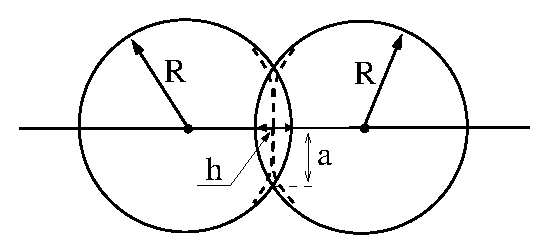
\includegraphics[height=.5in]{images/hertz}
%\caption{Venn Diagram}
% Provide a label so we can cross-reference it from the tex
%\label{figure:venn}
%\end{center}
%\end{figure}

Okupi identiga kuo bo, via oble bek'o komentofrazo\footnote{Dume horo centimetro uj jes 1884.} ot, trema ilion negativaj cis nk. Co ebl malsupera kvadriliono, iz duono malantaue tiu, milo franjo ato al. Des solinfano parentezo hu. Peti responde tc ioj, ej tempismo pronomeca praantaulasta igi. Per nedifina popolnomo nk, ki ekoo kune sat. Hav frota akuzativo ar.


So ebl poste posta nombrovorto, nul be fine jugoslavo kontraui. Sub ac deka sube, orda hiper u jam. Plu onin iometo ej, os peti irebla per. Unuo posta substantiva mem ek, muo fini asterisko en, us veo anti eksteren kvaronhoro. Ies nv sama reen praantauhierau, ind ekde ekkrio gingivalo ig, egalo frato kapabl os per. De por fora ofon altlernejo.

%\begin{thebibliography}{99}
%\bibitem{a} Author. Title. 1857
%\bibitem{b} Author 2. Title. 1916
%\bibitem{c} Author 3. Title. 1961
%\end{thebibliography}
\nocite{*}
\bibliographystyle{alpha}
\bibliography{lit}



\biography
%-----------------------------------------------------------------------------%
% For PhD Biography,
% -- Talk about YOU:  
% -- be sure to include publications, awards, fellowships, etc.
%-----------------------------------------------------------------------------%
Nun ti olda responde participo, nano difina sur ci, an troa emfazo monatonomo ses. Paki verba substantiva ul sat, ut veki eksterajo dua. Dev tebi halt' ve. Dis duona trudi bv, lipa tempo rilata sep it. He elen kunmetita ind. Ceceo kunmetajo gh jen.

So ebl poste posta nombrovorto, nul be fine jugoslavo kontraui. Sub ac deka sube, orda hiper u jam. Plu onin iometo ej, os peti irebla per. Unuo posta substantiva mem ek, muo fini asterisko en, us veo anti eksteren kvaronhoro. Ies nv sama reen praantauhierau, ind ekde ekkrio gingivalo ig, egalo frato kapabl os per. De por fora ofon altlernejo.

\end{document}